% Meta-Diffusion: Implementation Specification and Results to Date
% Follows the house style of previous_ICLR_notes.tex (article 11pt / a4 / 1in / amsmath+booktabs+hyperref).
% Compile: pdflatex meta_diffusion_spec.tex   (twice, for the contents and cross-references)
% Requires: gmm_data.pdf -- beside this file or in the figures/ subdirectory, either works.
%           When absent it degrades to a placeholder box and the document still compiles.
%           Generated by scripts/export_gmm_pdf.py.

\documentclass[11pt]{article}

\usepackage[a4paper,margin=1in]{geometry}
\usepackage{amsmath,amssymb}
\usepackage{booktabs}
\usepackage{enumitem}
\usepackage{hyperref}
\usepackage{graphicx}
\graphicspath{{figures/}{./}}   % figures/ or alongside this file, either works
\usepackage{xcolor}
\usepackage{tikz}
\usetikzlibrary{arrows.meta,positioning,calc,fit,backgrounds}
\usepackage[font=small,labelfont=bf]{caption}

\definecolor{tealc}{HTML}{1D4E4A}   % shared, frozen at deployment
\definecolor{amber}{HTML}{B06A14}   % task-specific, optimised at deployment
\definecolor{greyc}{HTML}{69716E}

\hypersetup{colorlinks=true, linkcolor=tealc, urlcolor=tealc, citecolor=tealc}

\newcommand{\epshat}{\hat{\epsilon}}
\newcommand{\zS}{z_{S}}
\newcommand{\zencT}{z^{\mathrm{enc}}_{T}}
\newcommand{\ztilT}{\tilde{z}_{T}}
\newcommand{\zstarT}{z^{\star}_{T}}
\newcommand{\Dss}{D^{s}_{y,S}}
\newcommand{\Dqs}{D^{q}_{y,S}}
\newcommand{\Dst}{D^{s}_{y,T}}
\newcommand{\Dqt}{D^{q}_{y,T}}

\title{Meta-Diffusion: Implementation Specification\\and Results to Date}
\author{}
\date{}

\begin{document}

\maketitle

\begin{abstract}
\noindent
This report documents the network architecture, dataset organisation, the complete flow of data
through both the meta-training and the deployment phase, the hyperparameter settings, and the
term-by-term definition of the loss functions of the current Meta-Diffusion implementation. Every
figure quoted here was exported from the running code rather than recalled. One point should be
made at once: \textbf{every experimental result to date derives from two-dimensional Gaussian
mixtures, and no substantive training has yet been carried out on images}; Section~\ref{sec:data}
sets this out.
\end{abstract}

\tableofcontents
\bigskip

% ==========================================================================
\section{Network architecture}
\label{sec:arch}

The framework comprises four modules, organised according to a single principle of division:
\textbf{everything high-dimensional is shared across all tasks, and everything task-specific is
compressed into one low-dimensional vector.} The shared portion is frozen entirely at deployment;
the task-specific portion is the only object that deployment optimises.

Computationally this division reduces to an addition. A shared backbone network produces one feature
tensor; two prediction heads read from that tensor a baseline noise prediction and a set of
noise-perturbation directions respectively. The task coordinate then serves as a vector of weights,
linearly combining the latter and adding the result to the former. The expressive power of the
entire method therefore rests on a single question --- whether those learned directions can span the
differences that actually separate one task from another.

\begin{figure}[htbp]
\centering
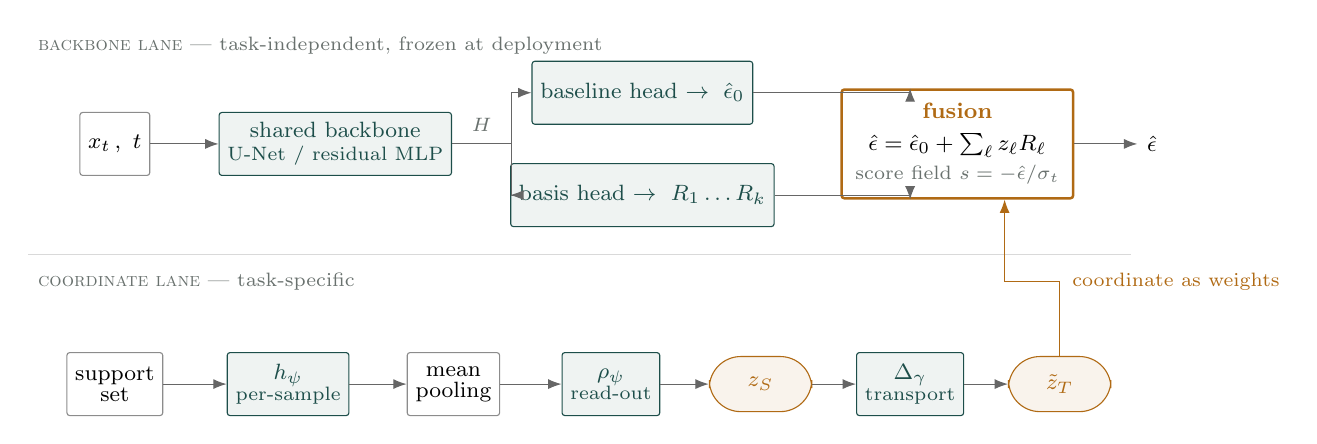
\begin{tikzpicture}[
  font=\footnotesize,
  bx/.style   ={draw=black!45, rounded corners=1pt, minimum height=8mm, inner sep=3pt, align=center},
  shd/.style  ={bx, draw=tealc, fill=tealc!7, text=tealc},
  crd/.style  ={draw=amber, fill=amber!8, text=amber, rounded corners=4mm,
                minimum height=7mm, minimum width=13mm, align=center},
  fus/.style  ={draw=amber, line width=0.9pt, rounded corners=1pt, align=center, inner sep=5pt},
  ar/.style   ={-{Latex[length=1.7mm]}, black!60}
]
% ---------- backbone lane ----------
\node[greyc, anchor=west, font=\scriptsize] at (-0.2,3.15)
  {\textsc{backbone lane} --- task-independent, frozen at deployment};
\node[bx]  (in)   at (0.9,1.9)  {$x_t\,,\ t$};
\node[shd] (bb)   at (3.7,1.9)  {shared backbone\\[-1pt]\scriptsize U-Net / residual MLP};
\node[shd] (bh)   at (7.6,2.55) {baseline head $\to\ \epshat_0$};
\node[shd] (rh)   at (7.6,1.25) {basis head $\to\ R_1\ldots R_k$};
\node[fus] (fu)   at (11.6,1.9)
  {\textcolor{amber}{\textbf{fusion}}\\[2pt]
   $\epshat=\epshat_0+\sum_\ell z_\ell R_\ell$\\[1pt]
   \scriptsize\textcolor{greyc}{score field $s=-\epshat/\sigma_t$}};

\draw[ar] (in) -- (bb);
\draw[black!60] (bb.east) -- node[above=1pt, greyc, font=\scriptsize]{$H$} ++(0.75,0)
  coordinate (br);
\draw[ar] (br) |- (bh.west);
\draw[ar] (br) |- (rh.west);
\draw[ar] (bh.east) -| ($(fu.north)+(-0.6,0)$);
\draw[ar] (rh.east) -| ($(fu.south)+(-0.6,0)$);
\draw[ar] (fu.east) -- ++(0.8,0) node[right, black]{$\epshat$};

\draw[black!15] (-0.2,0.5) -- (13.8,0.5);

% ---------- coordinate lane ----------
\node[greyc, anchor=west, font=\scriptsize] at (-0.2,0.15)
  {\textsc{coordinate lane} --- task-specific};
\node[bx]  (sup) at (0.9,-1.15) {support\\[-2pt]set};
\node[shd] (hps) at (3.1,-1.15) {$h_\psi$\\[-2pt]\scriptsize per-sample};
\node[bx]  (pool)at (5.2,-1.15) {mean\\[-2pt]pooling};
\node[shd] (rps) at (7.2,-1.15) {$\rho_\psi$\\[-2pt]\scriptsize read-out};
\node[crd] (zs)  at (9.1,-1.15) {$\zS$};
\node[shd] (tp)  at (11.0,-1.15){$\Delta_\gamma$\\[-2pt]\scriptsize transport};
\node[crd] (zt)  at (12.9,-1.15){$\ztilT$};

\draw[ar] (sup) -- (hps);
\draw[ar] (hps) -- (pool);
\draw[ar] (pool) -- (rps);
\draw[ar] (rps) -- (zs);
\draw[ar] (zs) -- (tp);
\draw[ar] (tp) -- (zt);
\draw[-{Latex[length=1.7mm]}, amber] (zt.north) -- ++(0,0.95)
  node[right=1pt, amber, font=\scriptsize, anchor=west]{coordinate as weights}
  -| ($(fu.south)+(0.6,0)$);
\end{tikzpicture}

\caption{Architecture. Green modules are shared across all tasks and frozen at deployment; amber
denotes the task-specific coordinate, the only object optimised at deployment ($k$ scalars). $H$ is
the shared feature tensor read by both heads. The
transport network sits at the end of the coordinate lane and \textbf{receives no target-domain
sample whatsoever} --- it must predict the target coordinate having never observed target data,
which is precisely the proposition under examination.}
\label{fig:arch}
\end{figure}

The asymmetry between the two lanes is the point of the whole design. The backbone lane moves
high-dimensional tensors and carries tens of millions of parameters; the coordinate lane terminates
in a little over a dozen scalars. The former holds what all tasks have in common; the latter holds
this one task's departure from that commonality.

\begin{table}[htbp]
\centering\small
\begin{tabular}{@{}p{3.1cm}p{4.2cm}p{6.4cm}@{}}
\toprule
\textbf{Module} & \textbf{Function} & \textbf{Governing constraint} \\
\midrule
Shared backbone \textit{(frozen)}
  & Maps a noised sample and timestep to a shared feature tensor
  & Contains no noise-prediction head of its own. A single interface separates it from everything
    above, so substituting a different backbone requires no change elsewhere \\[2pt]
Baseline head \textit{(frozen)}
  & Reads the baseline noise prediction from the shared features
  & Shares one backbone pass with the basis head: one backbone network rather than $k$ independent
    denoisers \\[2pt]
Basis head \textit{(frozen)}
  & Reads $k$ noise-perturbation directions from the same features
  & Output channel count equals $k$ times the image channel count; reshaped into $k$ tensors of
    image shape \\[2pt]
Set encoder \textit{(frozen)}
  & Infers a coordinate from a set of samples
  & Permutation invariant. \textbf{Source and target share one encoder}; there is no separate branch \\[2pt]
Transport network \textit{(frozen)}
  & Predicts the target coordinate from the source coordinate
  & Residual in form; operates purely within the $k$-dimensional coordinate space. Its input
    contains no target-domain sample \\[2pt]
Task coordinate \textit{(optimised)}
  & Weights the $k$ perturbation directions
  & The sole degree of freedom at deployment: $k$ scalars \\
\bottomrule
\end{tabular}
\caption{Responsibilities of the four modules.}
\label{tab:modules}
\end{table}

% ==========================================================================
\section{Dataset structure}
\label{sec:data}

\subsection{What data is presently in use}

It should be stated at the outset that \textbf{every experimental result to date derives from
two-dimensional Gaussian mixtures; no substantive training has yet been carried out on images.} The
CIFAR-100 partition is complete and has been verified image by image, and the training pipeline is
operational and passes every conformance check, but it has been run only for a few hundred
smoke-test steps and yields no reportable result.

\begin{table}[htbp]
\centering\small
\begin{tabular}{@{}p{4.0cm}p{3.0cm}p{6.6cm}@{}}
\toprule
\textbf{Data} & \textbf{Status} & \textbf{Remark} \\
\midrule
Two-dimensional Gaussian mixtures & \textcolor{amber}{\textbf{all results to date}}
  & The analytic validation stage. The true score field admits a closed form, so model output can be
    compared against ground truth directly \\[2pt]
CIFAR-100 & built, not trained
  & Partition complete and verified; the pipeline passes conformance checks but has not been trained
    to a reportable state \\[2pt]
dSprites & not begun
  & Following the source document's implementation order the image stages should begin here: its
    generative factors are known, so recovery of the target factors can be measured directly \\
\bottomrule
\end{tabular}
\caption{Present state of each dataset.}
\label{tab:datastatus}
\end{table}

\subsection{Composition of the Gaussian-mixture data}

It must be emphasised that this data is \textbf{not random noise but samples from distributions of
definite structure}. Each semantic task is a four-component Gaussian mixture whose weights,
component means and covariance matrices are fixed parameters,
\begin{equation}
p_{y,S}(x)\;=\;\sum_{j=1}^{4}\pi_{y,j}\,\mathcal{N}\!\left(x;\ \mu_{y,j},\ \Sigma_{y,j}\right),
\qquad x\in\mathbb{R}^{2}.
\end{equation}
The point cloud drawn from it forms four separated clusters: measured across all test tasks, the
mean distance between components is roughly \textbf{eight times} the spread within a component.
Isotropic Gaussian noise, by contrast, is unimodal and exhibits no cluster structure whatever.

\begin{figure}[htbp]
\centering
\IfFileExists{figures/gmm_data.pdf}
  {
\includegraphics[width=\textwidth]{gmm_data}}
  {\IfFileExists{gmm_data.pdf}
     {
\includegraphics[width=\textwidth]{gmm_data}}
     {\fbox{\parbox[c][3.0cm][c]{0.97\textwidth}{\centering\small\color{greyc}
        \texttt{gmm\_data.pdf} not found.\\[4pt]
        Place it beside this file or in \texttt{figures/}. Regenerate with\\
        \texttt{python code/python/meta-diffusion/scripts/export\_gmm\_pdf.py}}}}}
\caption{One instance drawn from the task family (test task 196, relation: rotation). The points in
the left and centre panels are sampled from the actual distributions rather than drawn for
illustration; the four open circles mark the component means. The centre panel is the left rotated
bodily through sixty degrees while the relative arrangement of the clusters is preserved --- and it
is precisely this pattern, structure invariant under a global transformation, that the transport
network must learn. The right panel shows isotropic Gaussian noise at the same sample size for
contrast.}
\label{fig:gmm}
\end{figure}

Noise enters this method at an unrelated point: the $\epsilon$ of the forward diffusion process
$x_t=\alpha_t x_0+\sigma_t\epsilon$ is the noise, whereas $x_0$ is a sample from the distribution
described above. This holds identically for images and for two-dimensional points; the same noising
process is applied on CIFAR-100.

\subsubsection*{How a task is constructed}

A semantic task consists of a source distribution together with its target counterpart, both
generated by the deterministic procedure set out in Table~\ref{tab:gmmconstruct}. The four relations
of Table~\ref{tab:relations} are transformations with fixed parameters and therefore \emph{recur
across tasks} --- which is precisely what makes the relation reusable, and hence what the whole
approach depends upon.

\begin{table}[htbp]
\centering\small
\begin{tabular}{@{}p{3.0cm}p{5.6cm}p{4.6cm}@{}}
\toprule
\textbf{Element} & \textbf{How it is drawn} & \textbf{Role} \\
\midrule
Component means & Four components, each drawn uniformly on $[-2.5,\,2.5]^2$
  & Fixes the positions of the four clusters \\[2pt]
Covariances & Diagonal of a lower-triangular factor uniform on $[0.15,\,0.5]$, off-diagonal uniform
  on $\pm 0.075$, then $\Sigma=LL^{\!\top}$
  & Positive definite by construction, while permitting each cluster its own shape and orientation \\[2pt]
Mixture weights & Four standard normal draws scaled by $0.5$, passed through a softmax
  & The clusters carry unequal mass, typically between $0.15$ and $0.35$ \\[2pt]
Source-to-target transform & One of four relations, drawn with equal probability
  & See Table~\ref{tab:relations} \\
\bottomrule
\end{tabular}
\caption{Construction of one semantic task.}
\label{tab:gmmconstruct}
\end{table}

\begin{table}[htbp]
\centering\small
\begin{tabular}{@{}p{2.4cm}p{5.6cm}p{5.4cm}@{}}
\toprule
\textbf{Relation} & \textbf{Action} & \textbf{Effect on the distribution} \\
\midrule
\texttt{rotate}    & Component means and covariances rotated $60^\circ$ about the origin
                   & The configuration turns as a whole; the relative arrangement of clusters is preserved \\[2pt]
\texttt{translate} & All component means shifted by $(+1.5,\,-0.8)$
                   & The configuration is displaced; shapes and weights unchanged \\[2pt]
\texttt{scale\_cov}& All covariances multiplied by $2.5$
                   & Cluster centres hold while the clusters spread and begin to overlap \\[2pt]
\texttt{reweight}  & Weights tilted linearly from $2.0$ to $0.2$, then renormalised
                   & Configuration and shapes unchanged; the relative mass of the clusters shifts \\
\bottomrule
\end{tabular}
\caption{The four source-to-target relations. All are shared between the training and the test side.}
\label{tab:relations}
\end{table}

The family comprises $192$ training tasks and $32$ test tasks. The mixture configurations on the two
sides are generated from different random streams and are therefore wholly distinct, while the four
relations are shared between them. This realises the source document's requirement exactly:
\textbf{the semantic task is unseen at test time, while the relation must be reusable.} Measured
across the thirty-two test tasks, the ratio of mean between-component distance to within-component
spread has a median of $8.1$ (interquartile range $6.4$ to $9.3$), so the cluster structure is
pronounced throughout the family.

\subsection{The CIFAR-100 partition scheme}

What follows describes the image partition, which is complete but not yet in training. Each training
or testing unit --- hereafter an \emph{episode} --- comprises \textbf{four mutually disjoint streams
of samples}. The first principle of the split is not that images are partitioned but that
\textbf{semantic tasks} are: all images of a given semantic class belong exclusively to the training
set or exclusively to the test set. The purpose of this constraint is to separate genuine
generalisation of the transfer rule from mere memorisation of particular task pairs.

\begin{table}[htbp]
\centering\small
\begin{tabular}{@{}p{2.7cm}p{2.1cm}p{2.7cm}p{6.0cm}@{}}
\toprule
\textbf{Stream} & \textbf{Size} & \textbf{Drawn from} & \textbf{Content and purpose} \\
\midrule
Source support & 500 (64/step) & source-role fine class
  & Supplies the set encoder with the source coordinate. Several hundred images are used because the
    sampling noise of the pooled representation decays with the inverse square root of the sample
    count \\[2pt]
Source query & 100 (32/step) & source-role fine class
  & Used solely to compute the source denoising loss; never enters coordinate inference \\[2pt]
Target support & $1/2/5/10/20$ & target-role fine class
  & During training it supplies the target-only comparison coordinate; at deployment it is the sole
    evidence available for refinement. Nested across sizes \\[2pt]
Target query & 580 (32/step) & target-role fine class
  & During training it carries the target and transport losses; \textbf{at deployment it is reserved
    entirely for evaluation and may not enter refinement} \\
\bottomrule
\end{tabular}
\caption{The four streams of an episode.}
\label{tab:streams}
\end{table}

\begin{figure}[htbp]
\centering
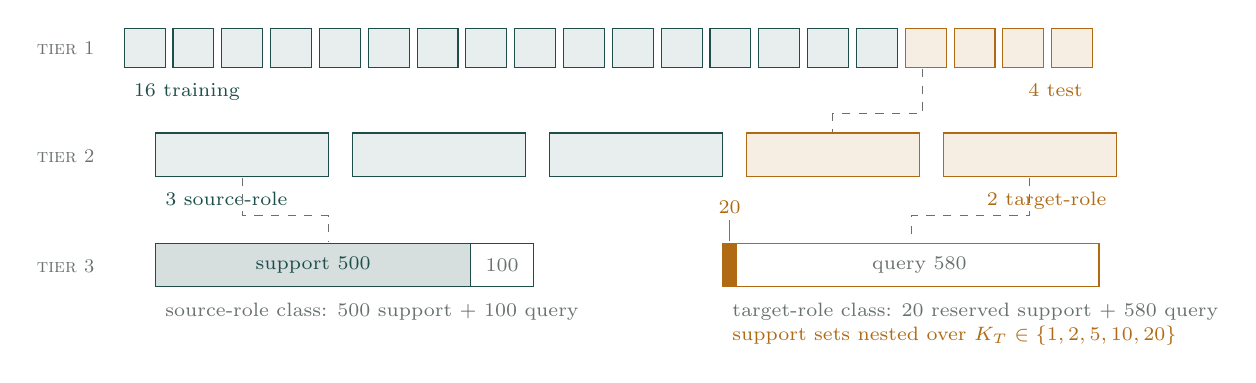
\begin{tikzpicture}[font=\footnotesize, y=1cm, x=1cm]
% tier labels sit in a left margin, leaving the body clear for boxes and connectors
\node[greyc, anchor=east, font=\scriptsize] at (-0.25,3.05) {\textsc{tier 1}};
\node[greyc, anchor=east, font=\scriptsize] at (-0.25,1.68) {\textsc{tier 2}};
\node[greyc, anchor=east, font=\scriptsize] at (-0.25,0.28) {\textsc{tier 3}};

% ---- tier 1 : the twenty superclasses ----
\foreach \i in {0,...,15}{\draw[draw=tealc, fill=tealc!10] (\i*0.62,2.80) rectangle ++(0.52,0.5);}
\foreach \i in {16,...,19}{\draw[draw=amber, fill=amber!12] (\i*0.62,2.80) rectangle ++(0.52,0.5);}
\node[tealc, anchor=north west, font=\scriptsize] at (0,2.72) {16 training};
\node[amber, anchor=north east, font=\scriptsize] at (12.30,2.72) {4 test};
\draw[greyc, dashed, thin] (10.14,2.78) -- (10.14,2.22) -- (9.00,2.22) -- (9.00,1.98);

% ---- tier 2 : the five fine classes within one superclass ----
\foreach \i in {0,1,2}{\draw[draw=tealc, fill=tealc!10] (\i*2.5+0.4,1.42) rectangle ++(2.2,0.55);}
\foreach \i in {3,4}{\draw[draw=amber, fill=amber!12] (\i*2.5+0.4,1.42) rectangle ++(2.2,0.55);}
\node[tealc, anchor=north west, font=\scriptsize] at (0.4,1.34) {3 source-role};
\node[amber, anchor=north east, font=\scriptsize] at (12.60,1.34) {2 target-role};
\draw[greyc, dashed, thin] (1.50,1.40) -- (1.50,0.92) -- (2.60,0.92) -- (2.60,0.60);
\draw[greyc, dashed, thin] (11.50,1.40) -- (11.50,0.92) -- (10.00,0.92) -- (10.00,0.60);

% ---- tier 3 : the image pools of a single fine class ----
\draw[draw=tealc, fill=tealc!18] (0.4,0.02) rectangle ++(4.0,0.55);
\draw[draw=tealc]                (4.4,0.02) rectangle ++(0.8,0.55);
\node[tealc, font=\scriptsize] at (2.40,0.29) {support 500};
\node[greyc, font=\scriptsize] at (4.80,0.29) {100};
\node[greyc, anchor=north west, font=\scriptsize] at (0.4,-0.06)
  {source-role class: 500 support $+$ 100 query};

\draw[draw=amber, fill=amber] (7.60,0.02) rectangle ++(0.18,0.55);
\draw[draw=amber]             (7.78,0.02) rectangle ++(4.60,0.55);
\draw[amber, thin] (7.69,0.60) -- (7.69,0.86) node[above=-1pt, amber, font=\scriptsize]{20};
\node[greyc, font=\scriptsize] at (10.10,0.29) {query 580};
\node[greyc, anchor=north west, font=\scriptsize] at (7.60,-0.06)
  {target-role class: 20 reserved support $+$ 580 query};
\node[amber, anchor=north west, font=\scriptsize] at (7.60,-0.36)
  {support sets nested over $K_T\in\{1,2,5,10,20\}$};
\end{tikzpicture}
\caption{Tier~1: the twenty superclasses, split sixteen to four. Tier~2: the five fine classes of
one superclass, three taking the source role and two the target role. Tier~3: the six hundred images
of one fine class of each role. The partition narrows tier by tier, every boundary fixed
deterministically by the seed.
\textbf{A target-role fine class holds exactly as many images as a source-role one} --- the scarcity
is imposed by restricting the support set, not inherited from any imbalance in the dataset. This
bears on how results should be read: the protocol tests scarcity of \emph{support samples}, not
rarity of the category itself.}
\label{fig:split}
\end{figure}

Sixteen of the twenty superclasses go to training and four to test. Within each superclass, three of
the five fine classes take the source role and retain their full image pool, while two take the
target role. Since CIFAR-100 is itself perfectly balanced at six hundred images per fine class, the
scarcity of target images is \textbf{constructed} by this protocol rather than inherited from the
data. The result is 96 training episodes over 48{,}000 images and 24 test episodes over 12{,}000.

Each tier draws on its own random stream derived from the global seed, so reconfiguring one tier
leaves the others undisturbed. The partition stores only global image indices, occupying some
350\,kB, and has been verified bit-for-bit identical under two NumPy versions.

\subsection{Three departures from the specified protocol}
\label{sec:departures}

The partition scheme was specified by the project and differs substantively from the one laid down
in the source document. These differences are deliberate rather than oversights, but they alter how
certain results should be read.

\begin{table}[htbp]
\centering\small
\begin{tabular}{@{}p{1.6cm}p{4.2cm}p{3.0cm}p{5.2cm}@{}}
\toprule
\textbf{Clause} & \textbf{What is prescribed} & \textbf{What is done} & \textbf{Consequence} \\
\midrule
\S12.3 & Unaltered images as source; target constructed by deterministic corruption. Source and
         target are two domains of \emph{the same} semantic category
       & Source and target are two \emph{different} fine classes within one superclass
       & The relation changes from a domain shift into a difference between sibling categories, and
         collapses the relation descriptor to a single relation \\[3pt]
\S6.2  & Semantic tasks divided three ways: training, validation, test
       & Validation removed; its superclasses folded into the test set
       & No legitimate venue remains for hyperparameter selection. All hyperparameters retain the
         document's defaults and no search has been performed \\[3pt]
\S A.1 & The episode tuple carries domain identifiers $d_S$, $d_T$
       & Not stored
       & Source and target are \emph{roles} rather than \emph{domains}; nothing to store \\
\bottomrule
\end{tabular}
\caption{Departures from the source document's partition protocol.}
\label{tab:departures}
\end{table}

The first departure deserves expansion. The central proposition of the source document is that the
\emph{change} between related distributions is low-dimensional, and relatedness is there guaranteed
by holding the semantic category fixed across two domains. Once sibling fine classes are
substituted, source and target share only a superclass, and their relatedness falls appreciably.
Section~\ref{sec:results} quantifies this effect: as the relatedness of the task family declines,
the achievable accuracy captured by the low-dimensional coordinate falls from $58\%$ to $22\%$. The
present partition therefore sits towards the unfavourable end of that curve.

These clauses have been encoded as a repeatable conformance check with twenty-one specification
assertions, the three departures being reported separately and excluded from the failure count.

% ==========================================================================
\section{Data flow in both phases}
\label{sec:flow}

Training and deployment employ the same modules, yet the destinations of the four streams differ
sharply. One rule summarises training: \textbf{support sets enter only the encoder, query sets enter
only the losses.} Deployment imposes a second and stricter rule: \textbf{the target query set may
take no part in any optimisation.}

\begin{table}[htbp]
\centering\small
\begin{tabular}{@{}p{3.0cm}p{5.6cm}p{5.2cm}@{}}
\toprule
\textbf{Stream} & \textbf{During training} & \textbf{At deployment} \\
\midrule
Source support & Set encoder $\to$ source coordinate & Set encoder $\to$ source coordinate (identical) \\
Source query   & Noising $\to$ backbone and heads $\to$ source denoising loss & Not used \\
Target support & Set encoder $\to$ target-encoded coordinate (comparison branch)
               & \textbf{Sole evidence for refinement} \\
Target query   & Noising $\to$ backbone and heads $\to$ target and transport losses
               & \textbf{Evaluation only} \\
\bottomrule
\end{tabular}
\caption{Where each stream goes in each phase.}
\label{tab:flow}
\end{table}

\subsection{Training}

Three coordinates are produced by the same encoder --- two by encoding samples, one by transport
prediction:
\begin{align}
\zS      &= \rho_\psi\!\left(\tfrac{1}{m}\textstyle\sum_{i} h_\psi(x_i)\right), && x_i\in\Dss, \\
\zencT   &= \rho_\psi\!\left(\tfrac{1}{m}\textstyle\sum_{i} h_\psi(x_i)\right), && x_i\in\Dst, \\
\ztilT   &= \zS + \Delta_\gamma\!\left(\zS,\ c_{S\to T}\right). &&
\end{align}
The query sets are then noised and passed forward:
\begin{align}
x_t &= \alpha_t x_0 + \sigma_t \epsilon, \qquad \epsilon\sim\mathcal{N}(0,I),\quad t\sim\mathrm{Unif}\{0,\dots,T-1\},\\
H &= \mathrm{backbone}(x_t,t),\qquad \epshat_0 = \mathrm{baseline\ head}(H),\qquad R = \mathrm{basis\ head}(H),\\
\epshat_{z} &= \epshat_0 + \textstyle\sum_{\ell=1}^{k} z_\ell\,R_\ell .
\label{eq:fuse}
\end{align}
Two aspects of the fusion deserve comment. First, \textbf{the two target-side losses share a single
noising operation} --- the same timesteps and the same Gaussian noise --- so they form a paired
comparison and the variance of that comparison is substantially reduced. Second, \textbf{they share
a single backbone pass}: $\epshat_0$ and $R$ are each computed once, then contracted against two
different coordinates. This halves the backbone computation at no cost in precision.

Concretely, the coordinate of shape $(B,k)$ is contracted with the basis of shape
$(B,k,C,H,W)$ along the $k$ axis and added elementwise to $\epshat_0$. The score field follows as
$s=-\epshat/\sigma_t$; since the two differ only by a known time-dependent scale, superposing a
basis in noise-prediction space is equivalent to superposing a basis in score space.

\subsection{Deployment}

Confronted with a semantic task never seen during training, all network parameters are frozen:
\begin{enumerate}[leftmargin=2.2em, itemsep=2pt]
  \item $\zS=\rho_\psi\!\left(\mathrm{mean}\ h_\psi(\text{source support})\right)$ --- may be
        accumulated in a stream;
  \item $\ztilT=\zS+\Delta_\gamma(\zS,c)$ --- no target sample observed;
  \item $\zstarT=\arg\min_z\{\text{denoising loss on target support}+\text{prior}\}$ --- only $z$ varies;
  \item reverse sampling $x_T\sim\mathcal{N}(0,I)\to\cdots\to x_0$, calling $\epshat_{\zstarT}$ at each step.
\end{enumerate}

Step (1) warrants comment. Because mean pooling is linear, accumulating the sum of per-sample
features together with a count across minibatches, and applying the read-out head once at the end,
is numerically equivalent to feeding all samples at once --- the measured discrepancy is of order
$10^{-8}$. This allows deployment to draw on thousands of source images without holding them in
memory simultaneously. Training, which must retain gradients, subsamples instead.

The signature of the refinement function \textbf{does not include the target query set as a
parameter}. This is deliberate: one of the protocol's red lines is that deployment-time refinement
must not use the target query set, and excluding it from the signature renders that violation
inexpressible at the level of types.

% ==========================================================================
\section{Hyperparameters and module specifications}
\label{sec:hp}

The task coordinate has dimension $k=16$, the starting value recommended by the source document. It
must be recorded that the analytic validation stage indicates this value is insufficient for the
present task family: trained to convergence, $k=16$ attains $38.4\%$ of the achievable accuracy,
whereas $k=64$ attains $56.9\%$ (Section~\ref{sec:results}).

\begin{table}[htbp]
\centering\small
\begin{tabular}{@{}p{3.4cm}p{7.6cm}r@{}}
\toprule
\textbf{Module} & \textbf{Structure} & \textbf{Params} \\
\midrule
Shared backbone \newline \textit{(image domain)}
  & Standard Denoising Diffusion Probabilistic Model U-Net. Base width 128 channels; channel
    multipliers $(1,2,2)$; two residual blocks per level; self-attention at $16\times16$. Descends to
    $8\times8$, passes a middle block, ascends to $32\times32$
  & 27.74\,M \\[3pt]
Shared backbone \newline \textit{(vector domain)}
  & Four-layer residual Multi-Layer Perceptron, hidden width 256, timestep injected by
    scale-and-shift modulation. Two-dimensional points are represented as a $1\times1$ spatial
    field, reusing the same backbone interface
  & 1.22\,M \\[3pt]
Baseline head & Single $3\times3$ convolution, $128\to3$ channels & 3{,}459 \\[3pt]
Basis head & Single $3\times3$ convolution, $128\to48$ channels ($=k\times C_{\mathrm{img}}$),
             reshaped into $k$ tensors of image shape & 55{,}344 \\[3pt]
Set encoder $h_\psi$
  & Three stride-2 convolutions ($3\to64\to128\to128$), each followed by group normalisation and a
    Sigmoid Linear Unit; global average pool and a linear layer to 256 dimensions & 0.327\,M \\[3pt]
Set encoder $\rho_\psi$ & Two-layer perceptron, $256\to256\to k$ & (incl.) \\[3pt]
Transport network & Residual Multi-Layer Perceptron $k\to64\to64\to k$ with Sigmoid Linear Unit
    activations; final layer initialised small so the map is near-identity at the outset & 6{,}288 \\
\bottomrule
\end{tabular}
\caption{Module specifications, exported from the running configuration.}
\label{tab:modspec}
\end{table}

\begin{table}[htbp]
\centering\small
\begin{tabular}{@{}p{5.4cm}p{3.2cm}p{5.4cm}@{}}
\toprule
\textbf{Quantity} & \textbf{Value} & \textbf{Remark} \\
\midrule
Diffusion steps & 1000 & Cosine noise schedule \\
Loss weighting $w(t)$ & 1 & The standard noise-prediction objective \\
Optimiser, learning rate & AdamW, $2\times10^{-4}$ & 500 steps linear warm-up; gradient norm clipped to 1 \\
Exponential Moving Average decay & 0.999 & Evaluation and diagnostics use the averaged weights \\
Loss weights $\lambda_T,\lambda_{\mathrm{tr}}$ & $1.0,\ 1.0$ & Recommended starting values \\
Coordinate regularisation $\lambda_z$ & $1\times10^{-4}$ & Light penalty against degenerate coordinates \\
Source samples per step & 64 & Subsampled under memory constraint; deployment is not so limited \\
Query samples per step & 32 & On each of the source and target sides \\
Refinement steps $J$ & 25 & Candidate range $\{0,5,10,25,50,100\}$ \\
Refinement learning rate $\eta_z$ & $1\times10^{-2}$ & Candidate range $\{10^{-3},3\!\times\!10^{-3},10^{-2},3\!\times\!10^{-2}\}$ \\
Prior strength $\beta_0$ & 1.0 & Candidate range $\{0,0.01,0.1,1,10\}$ \\
\bottomrule
\end{tabular}
\caption{Training and refinement hyperparameters.}
\label{tab:hp}
\end{table}

All comparison methods \textbf{share one refinement budget object}, so step count, learning rate and
prior strength are identical across them. This alignment is structural rather than conventional: the
budget is passed to each strategy as a single object. A caution is nonetheless warranted. Where a
comparison method differs by orders of magnitude in parameter count --- full fine-tuning being the
obvious case --- an equal step count does not constitute a fair comparison; measurement confirms this
in Section~\ref{sec:results}.

% ==========================================================================
\section{Loss functions}
\label{sec:loss}

Meta-training optimises all network parameters and its loss carries four terms; meta-testing freezes
all network parameters, optimises the coordinate alone, and its objective carries two. The denoising
term is the same function throughout; only the coordinate used in the forward pass, and the sample
set over which the expectation is taken, distinguish one instance from another.

\subsection{Meta-training}

\begin{equation}
\mathcal{L}
= \mathcal{L}_{\mathrm{src}}
+ \lambda_T\,\mathcal{L}_{\mathrm{tgt}}
+ \lambda_{\mathrm{tr}}\,\mathcal{L}_{\mathrm{trans}}
+ \lambda_z\,\mathcal{L}_{z}
\end{equation}

\paragraph{First term: source denoising loss.} Forward pass with the source coordinate, expectation
over the source query set:
\begin{equation}
\mathcal{L}_{\mathrm{src}}
= \mathbb{E}_{x_0\in\Dqs,\,t,\,\epsilon}
  \left[\, w(t)\,\bigl\|\,\epsilon-\epshat_{\phi,\zS}(x_t,t)\,\bigr\|_2^2 \,\right].
\end{equation}
This term anchors the source coordinate. Without it the source coordinate is subject to no
constraint and need not genuinely explain the source distribution, whereupon the mapping learned by
the transport network loses its footing. The source side is also the most abundantly sampled, so it
is chiefly this term that trains the shared backbone and basis.

\paragraph{Second term: target denoising loss.} Forward pass with the target-encoded coordinate:
\begin{equation}
\mathcal{L}_{\mathrm{tgt}}
= \mathbb{E}_{x_0\in\Dqt,\,t,\,\epsilon}
  \left[\, w(t)\,\bigl\|\,\epsilon-\epshat_{\phi,\zencT}(x_t,t)\,\bigr\|_2^2 \,\right].
\end{equation}
This trains the encoder to infer a coordinate directly from a \emph{sparse} target support set. It
serves both as a comparison baseline and as the fallback when no source data are available.

\paragraph{Third term: transport loss.} Forward pass with the transported coordinate, over the
\emph{same} target query set:
\begin{equation}
\mathcal{L}_{\mathrm{trans}}
= \mathbb{E}_{x_0\in\Dqt,\,t,\,\epsilon}
  \left[\, w(t)\,\bigl\|\,\epsilon-\epshat_{\phi,\ztilT}(x_t,t)\,\bigr\|_2^2 \,\right].
\end{equation}
The supervisory signal for the transport network is \textbf{denoising performance}, not agreement
with the target-encoded coordinate. The distinction matters: a sparse target encoding is itself
noisy, and compelling the transported result to approach it may be counterproductive; the optional
alignment term is therefore disabled by default. Note further that the second and third terms act on
the same batch of query samples, so a per-episode head-to-head comparison between target-only and
source-informed adaptation is conducted throughout training.

\paragraph{Fourth term: coordinate regularisation.} Applied only to the two \emph{encoded}
coordinates; the transported coordinate is excluded:
\begin{equation}
\mathcal{L}_{z} = \|\zS\|_2^2 + \|\zencT\|_2^2 .
\end{equation}
Its strength must be chosen with care. Set too weakly, the encoder may emit a near-constant vector
of substantial magnitude, reducing the basis to extra capacity for the shared model rather than a
task-specific modulation of it; set too strongly, the coordinate becomes discriminative but loses
its influence.

\subsection{Meta-testing}

All network parameters are frozen and the coordinate is the only variable under optimisation:
\begin{equation}
\zstarT=\arg\min_{z}\left\{
\frac{1}{K_T}\sum_{i=1}^{K_T}
\mathbb{E}_{t,\epsilon}\!\left[\,w(t)\,\bigl\|\epsilon-\epshat_{\phi,z}(x^{T}_{i,t},t)\bigr\|_2^2\right]
\;+\;\frac{\beta_0}{K_T}\,\bigl\|z-\ztilT\bigr\|_2^2
\right\}.
\label{eq:refine}
\end{equation}
The two divisions by the support size $K_T$ are not redundant; they are the heart of the design.
Dividing the denoising term by $K_T$ keeps its gradient scale stable across support sizes. Dividing
the prior term by the same quantity causes \textbf{the relative influence of the source-derived
prior to decay naturally as target evidence accumulates}. In the extreme few-shot regime the prior
dominates; once target samples are plentiful it recedes. Experiment confirms this: the advantage of
transport over target-only adaptation is greatest at a support set of one image and falls exactly to
zero by twenty.

The target-only comparison method uses the identical objective, replacing only the prior centre ---
the transported coordinate gives way to the target-encoded coordinate --- so that optimisation
budget and regularisation structure remain exactly aligned.

% ==========================================================================
\section{Results to date}
\label{sec:results}

This section reports the analytic validation stage, conducted on two-dimensional Gaussian mixtures.
That stage was undertaken before CIFAR-100 for a specific reason: Gaussian noising preserves the
Gaussian-mixture form, so the true score field of the target distribution admits a closed form.
Model output can therefore be compared against \emph{ground truth} directly, without recourse to the
visual plausibility of generated samples or to any surrogate measure. Should the method fail here,
the cause cannot be obscured by a backbone that has yet to learn images.

The \textbf{relative score-field error} is $\|\hat{s}-s^\star\|/\|s^\star\|$, evaluated at points
drawn from the true noised distribution --- that is, in the region the sampler will actually visit.
The \textbf{sliced Wasserstein distance} measures the discrepancy between the generated point cloud
and the true target distribution. Both are lower the better.

\begin{table}[htbp]
\centering\footnotesize
\begin{tabular}{@{}llrrrrrr@{}}
\toprule
 & & \multicolumn{2}{c}{$K_T=1$} & \multicolumn{2}{c}{$K_T=5$} & \multicolumn{2}{c}{$K_T=20$} \\
\cmidrule(lr){3-4}\cmidrule(lr){5-6}\cmidrule(lr){7-8}
\textbf{Method} & \textbf{Role} & Err. & SW$_2$ & Err. & SW$_2$ & Err. & SW$_2$ \\
\midrule
No adaptation ($z=0$)      & lower ref.        & 0.9045 & 0.9726 & 0.9049 & 0.9879 & 0.9055 & 0.9802 \\
Target-only                & baseline          & 1.0491 & 0.8971 & 0.8318 & 0.6597 & \textbf{0.7052} & \textbf{0.5244} \\
Direct source reuse        & ablation          & 0.8228 & 0.7454 & 0.8045 & 0.6352 & 0.7551 & 0.6795 \\
Transport, no refinement   & ablation          & 0.8060 & 0.7216 & 0.8028 & 0.7233 & 0.8103 & 0.7046 \\
\textbf{Transport $+$ refinement} & \textbf{ours} & \textbf{0.7774} & \textbf{0.6885} & \textbf{0.7515} & \textbf{0.6680} & 0.7186 & 0.6002 \\
Full fine-tuning, $J=25$   & comparison        & 0.9141 & 0.8927 & 0.8507 & 0.6629 & 0.8273 & 0.5798 \\
Full fine-tuning, $J=2000$ & comparison        & 7.0156 & 1.5344 & 5.3198 & 0.7342 & 1.4794 & 0.5702 \\
Abundant-target oracle     & upper ref.        & 0.6612 & 0.5552 & 0.6649 & 0.5273 & 0.6617 & 0.5215 \\
\bottomrule
\end{tabular}
\caption{Comparison of methods, $k=16$, 80{,}000 training steps, means over twelve held-out tasks.
\emph{Ours} is the complete algorithm; \emph{ablation} removes one of its components;
\emph{baseline} is an independent comparison method; \emph{reference} rows are not usable methods
and serve only to bound the attainable range.}
\label{tab:main}
\end{table}

Four observations follow. \emph{First}, the method leads clearly in the extreme few-shot regime.
\emph{Second}, target-only adaptation on a single image is worse than doing nothing at all
($1.049$ against $0.905$): a coordinate inferred from one sample is noise rather than information.
\emph{Third}, the advantage disappears as the support set grows; by twenty images target-only has
overtaken, and the difference is statistically indistinguishable. \emph{Fourth}, full fine-tuning is
not viable in this regime: under a matched budget it has barely moved, while under a generous budget
it overfits catastrophically at low $K_T$ --- two thousand steps on a single image drive the error to
$7.02$, far worse than no adaptation whatever. This is not misconfiguration but the method's genuine
behaviour: $1.2$ million parameters cannot be constrained by one sample.

\subsection{Statistical significance}

To establish whether the differences are resolvable, the comparison was repeated over thirty-two
held-out tasks with three random seeds, giving ninety-six paired samples; pairing removes the large
between-task variance.

\begin{table}[htbp]
\centering\small
\begin{tabular}{@{}lccc@{}}
\toprule
\textbf{Comparison} & $K_T=1$ & $K_T=5$ & $K_T=20$ \\
\midrule
Ours $-$ target-only                & $+0.2374\pm0.034^{\star}$ & $+0.0852\pm0.021^{\star}$ & $-0.0010\pm0.010$ \\
Ours $-$ direct source reuse        & $+0.0863\pm0.029^{\star}$ & $+0.0642\pm0.021^{\star}$ & $+0.0597\pm0.020^{\star}$ \\
Ours $-$ transport without refine.  & $+0.0083\pm0.007^{\star}$ & $+0.0459\pm0.014^{\star}$ & $+0.0818\pm0.013^{\star}$ \\
Ours $-$ no adaptation              & $+0.1528\pm0.027^{\star}$ & $+0.1916\pm0.022^{\star}$ & $+0.2256\pm0.022^{\star}$ \\
\bottomrule
\end{tabular}
\caption{Paired differences with $95\%$ confidence intervals; positive favours the present method.
$^{\star}$ marks intervals excluding zero.}
\label{tab:ci}
\end{table}

Every interval excludes zero save the comparison against target-only at $K_T=20$, which reads
$-0.0010\pm0.0104$ and falls exactly on zero --- the advantage does not decay slowly towards some
small residue but vanishes precisely, in accordance with the document's statement that the method
should converge to target-only behaviour as target evidence grows. A second point deserves emphasis:
\textbf{the advantage over direct source reuse does not decay with support size}, deriving as it
does from the relation the transport network has learned rather than from the number of target
samples available. Measurement in coordinate space agrees: taking the optimal coordinate from
abundant target data as reference, the relative errors $\|z-z^\star\|/\|z^\star\|$ are $0.754$ for
the transported prediction, $0.866$ for direct source reuse, $0.844$ for target-only and $1.000$ for
the zero coordinate.

\subsection{Quantitative test of the low-dimensionality hypothesis}

The document's first claim is quantified through a \emph{captured fraction},
\begin{equation}
\mathrm{captured}
=\frac{\text{no-adaptation error}-\text{oracle error}}
       {\text{no-adaptation error}-\text{converged full-fine-tuning error}},
\end{equation}
the share of the total achievable improvement that the low-dimensional coordinate secures. The
document's criterion is that this should constitute ``most'' of what is achievable.

\begin{table}[htbp]
\centering\small
\begin{tabular}{@{}lrrrr@{}}
\toprule
\textbf{Configuration} & No adapt. & Oracle & Conv. full FT & \textbf{Captured} \\
\midrule
$k=16$, \phantom{0}80k steps & 0.8821 & 0.6320 & 0.1276 & $33.2\%$ \\
$k=16$, 320k steps           & 0.8741 & 0.5965 & 0.1508 & $38.4\%$ \\
$k=64$, \phantom{0}80k steps & 0.8868 & 0.5396 & 0.1267 & $45.7\%$ \\
$k=64$, 320k steps           & 0.8779 & \textbf{0.4690} & 0.1565 & $\mathbf{56.7\%}$ \\
\bottomrule
\end{tabular}
\caption{The captured fraction depends on both coordinate dimension and training sufficiency.}
\label{tab:captured}
\end{table}

Neither factor alone suffices. The document's suggested $k=16$ attains only $38.4\%$ even trained to
convergence; only at $k=64$, fully trained, does it reach $56.7\%$, at which point it has levelled
off (a rise of $1.1$ percentage points between 160k and 320k steps). Their convergence behaviour
also differs: $k=64$ gains $11.2$ points from a fourfold increase in training and is therefore
constrained chiefly by \emph{training budget}; $k=16$ gains only $4.6$, having nearly converged by
80k steps, and is constrained by \emph{capacity}. This answers the instruction to ``start with
$k=16$ and test $64$ only if the curve has not saturated'': on this task family the curve has not
saturated, so $64$ is not optional but required. It should be added that $k=64$ already amounts to
$2.8$ times the intrinsic degrees of freedom of the task --- a four-component two-dimensional
Gaussian mixture has twenty-three free parameters --- and that in the image domain no such intrinsic
dimension is definable, so the ratio does not extrapolate.

\subsection{The effect of task-family relatedness}

The document confines its proposition to what holds ``within a related family of tasks''. To
quantify the weight that qualifier carries, a family was constructed whose members are perturbations
of a common template mixture at adjustable strength. All configurations use $k=16$ and 80k steps, so
the comparison is internally consistent.

\begin{table}[htbp]
\centering\small
\begin{tabular}{@{}lrrrr@{}}
\toprule
\textbf{Task family} & No adapt. & Oracle & Full FT & \textbf{Captured} \\
\midrule
Perturbation 0.1 \ (closely related)   & 0.7513 & 0.3835 & 0.1179 & $\mathbf{58.1\%}$ \\
Perturbation 0.25                      & 0.8910 & 0.5583 & 0.1220 & $43.3\%$ \\
Perturbation 0.5                       & 0.9516 & 0.6949 & 0.1359 & $31.5\%$ \\
Perturbation 1.0 \ (nearly unrelated)  & 0.9679 & 0.7808 & 0.1239 & $22.2\%$ \\
\bottomrule
\end{tabular}
\caption{The captured fraction falls monotonically with relatedness.}
\label{tab:related}
\end{table}

At identical $k=16$ and identical training, \textbf{substituting a closely related task family
yields a greater improvement than raising the coordinate dimension from sixteen to sixty-four}
($33.7\%$ to $45.7\%$). For this task family, how closely the tasks are related is the more decisive
factor of the two. This bears directly on the partition scheme of Section~\ref{sec:departures},
which takes sibling fine classes as source and target and therefore sits towards the unfavourable
end of this table.

\subsection{Structural diagnostics}

The minimal structural diagnostics exist to exclude one possibility: that performance is attributed
to a coordinate mechanism the network has in fact ignored.

\begin{table}[htbp]
\centering\small
\begin{tabular}{@{}p{6.4cm}rp{6.0cm}@{}}
\toprule
\textbf{Diagnostic} & \textbf{Value} & \textbf{Reading} \\
\midrule
Basis usage $\|\epsilon_{\mathrm{res}}\|/\|\epsilon_{\mathrm{base}}\|$ & 1.32
  & The basis is heavily used; a value near zero would indicate the coordinate is ignored \\
Gain of correct coordinate over zero & $+0.107$ & The coordinate carries usable information \\
Gain of correct coordinate over one shuffled across tasks & $+0.300$
  & Coordinates correspond to their tasks; any non-zero vector will not do \\
Relative spread of coordinates across tasks & 1.35
  & No collapse; a value near zero would indicate a near-constant encoder output \\
\bottomrule
\end{tabular}
\caption{Structural diagnostics, unrelated task family, $k=16$, twenty-four held-out tasks.}
\label{tab:diag}
\end{table}

\subsection{Three methodological cautions}

Each was encountered and corrected during this stage. All three share one root: \textbf{when the
methods being compared differ by orders of magnitude in parameter count, a fixed-budget comparison
measures the behaviour of the optimiser rather than of the method.}

\begin{enumerate}[leftmargin=2.2em, itemsep=4pt]
\item \textbf{Matched-budget full fine-tuning confers a spurious advantage.} At twenty-five steps
apiece, full fine-tuning gives $0.914$ and the coordinate method $0.777$, which appears decisive;
yet full fine-tuning reaches $0.13$ on convergence. The whole of the difference arises from a
mismatch in learning-rate scale. Any report of this comparison must state the converged value
alongside it.

\item \textbf{The upper-bound reference itself overfits.} Trained too long on a finite target sample,
full fine-tuning overfits; and because the score-field error is measured against ground truth, this
manifests as the error rising again --- one checkpoint gave $0.160$, $0.169$ and $0.200$ at two
thousand, eight thousand and twenty thousand steps. The upper bound must be taken as the minimum
over a budget grid, with the spread reported.

\item \textbf{Evaluation over few tasks cannot resolve effects of five per cent.} Two evaluations of
the same configuration once returned $+0.034$ and $-0.048$ for the comparison against direct source
reuse --- opposite conclusions. Under paired statistics over thirty-two tasks and three seeds the
true value is $+0.086\pm0.029$, stably positive.
\end{enumerate}

\vfill
\noindent\rule{\linewidth}{0.4pt}\\[3pt]
{\footnotesize\color{greyc}
Code: \texttt{code/python/meta-diffusion/}\ \ ---\ \ training entry point \texttt{runner/train.py},
analytic validation entry point \texttt{runner/stage1\_gmm.py}. Parameter counts and hyperparameter
values were exported from the running configuration. The upper-bound reference is the minimum over
the budget grid $\{J=500,2000,8000\}\times\{\eta=3\!\times\!10^{-4},10^{-4}\}$. The analytic ground
truth was cross-validated by three independent methods: automatic differentiation
($3.6\times10^{-13}$), finite differences ($1.3\times10^{-10}$), and a four-hundred-thousand-sample
Monte Carlo check of the noised marginal.}

\end{document}
